\section{BPMN}

\begin{frame}{BPMN}
    \begin{itemize}
        \item Son las siglas para Business Process Modeling Notation.
	    \item Es un lenguaje para facilitar la comunicación de los procesos en forma clara, completa y eficiente.
	\end{itemize}
\end{frame}

\begin{frame}{Elementos de un diagrama BPMN}
    \begin{itemize}
        \item Un diagrama BPMN está compuesto por tres elementos básicos, que son los objetos de flujo (eventos, actividades y compuertas), además de objetos conectores y reglas de construcción. 
    \end{itemize}
\end{frame}

\subsection{Eventos}

\begin{frame}{Eventos}
    \begin{itemize}
        \item Representan algo que ocurre o puede ocurrir durante el curso del proceso.
        \item Suelen tener una causa o un resultado.
        \item De acuerdo con el momento en que afectan al flujo, se dividen en tres tipos:
        \begin{enumerate}
            \item Eventos de inicio.
            \item Eventos intermedios.
            \item Eventos de fin.
        \end{enumerate}
    \end{itemize}
\end{frame}

\begin{frame}{Eventos de inicio}
    \begin{itemize}
        \item Representa el disparador de un proceso. Todo proceso debe tener al menos un evento de inicio.
    \end{itemize}
    \begin{figure}
        \centering
        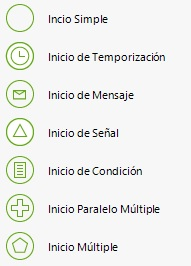
\includegraphics[scale=0.8]{images/event_start.jpg}
        %\caption{Caption}
        %\label{fig:my_label}
    \end{figure}
\end{frame}

\begin{frame}{Eventos intermedios}
    \begin{itemize}
        \item Ocurren a la mitad del proceso, forman parte directa del flujo del proceso.
    \end{itemize}
    \begin{figure}
        \centering
        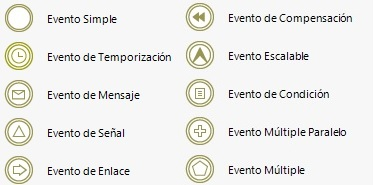
\includegraphics[scale=0.8]{images/event_intermediate.jpg}
        %\caption{Caption}
        %\label{fig:my_label}
    \end{figure}    
\end{frame}

\begin{frame}{Eventos de fin}
    \begin{itemize}
        \item Identifican el fin del proceso. 
        \item Todo proceso debe tener al menos un evento de fin, pero es común que tengan varios para dar claridad al tipo de terminación que tuvo el proceso.
    \end{itemize}
    \begin{figure}
        \centering
        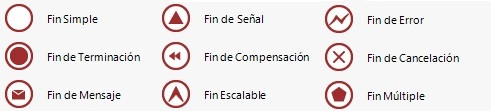
\includegraphics[scale=0.8]{images/event_final.jpg}
        %\caption{Caption}
        %\label{fig:my_label}
    \end{figure}
\end{frame}

\subsection{Actividades}

\begin{frame}{Actividades}
    \begin{itemize}
        \item Es un término genérico para el trabajo que se realiza en el proceso. 
        \item Representado por un rectángulo redondeado. 
        \item Puede ser:
            \begin{itemize}
                \item Tareas.
                \item Subprocesos.
            \end{itemize}
    \end{itemize}
    
\end{frame}

\begin{frame}{Tareas}
    \begin{itemize}
        \item Representan el trabajo que consume recursos de la organización.
        \item Cuando una actividad es completada la siguiente actividad inicia.
    \end{itemize}
    \begin{figure}
        \centering
        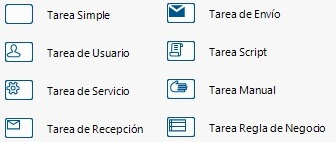
\includegraphics[scale=0.8]{images/task.jpg}
        %\caption{Caption}
        %\label{fig:my_label}
    \end{figure}
\end{frame}

\begin{frame}{Subprocesos}
    \begin{itemize}
        \item Es una actividad compuesta incluida dentro de un proceso.
        \item Incluye a su vez un conjunto de actividades y una secuencia lógica, por lo que dicha actividad puede ser analizada a nivel más fino.
    \end{itemize}
    \begin{figure}
        \centering
        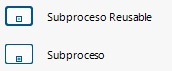
\includegraphics[scale=0.8]{images/subprocess.jpg}
        %\caption{Caption}
        %\label{fig:my_label}
    \end{figure}
\end{frame}

\subsection{Compuertas}

\begin{frame}{Compuertas}
    \begin{itemize}
        \item Controlan los puntos de divergencia y de convergencia del flujo.
    \end{itemize}
    \begin{figure}
        \centering
        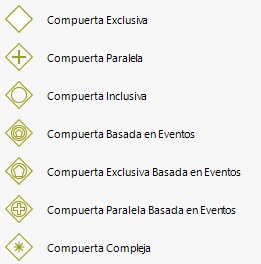
\includegraphics[scale=0.8]{images/gateway.jpg}
        %\caption{Caption}
        %\label{fig:my_label}
    \end{figure}
\end{frame}

\subsection{Objetos conectores}

\begin{frame}{Objetos conectores}
    \begin{itemize}
        \item Conectan los objetos de flujo de un proceso, y definen el orden de ejecución de las actividades. Pueden ser:
        \begin{itemize}
            \item Secuencia: Muestra el orden de los eventos, actividades, decisiones que se realizan dentro del proceso.
            \item Mensaje: Identifica el flujo de mensajes entre las distintas partes de los procesos.
            \item Asociación: Asocia artefactos con objetos de flujo.
        \end{itemize}
    \end{itemize}
    \begin{figure}
        \centering
        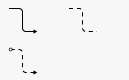
\includegraphics[scale=0.8]{images/flows.jpg}
        %\caption{Caption}
        %\label{fig:my_label}
    \end{figure}
\end{frame}

\subsection{Reglas}

\begin{frame}{Reglas}
    \begin{itemize}
        \item Un \textit{pool} contiene un único proceso y su nombre puede considerarse como el nombre del proceso.
        \item Los canales (\textit{lanes}) representan a cada uno de los participantes del proceso. Puede representar un área funcional, un cargo o un rol.
        \item Las fases se utilizan para delimitar las etapas distintas de un proceso, en donde se puede identificar una salida intermedia entre una etapa y la siguiente.
    \end{itemize}
    \begin{figure}
        \centering
        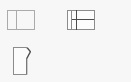
\includegraphics[scale=0.8]{images/rules.jpg}
        %\caption{Caption}
        %\label{fig:my_label}
    \end{figure}
\end{frame}